\section{Deadlock}

Il deadlock é un sotto problema rispetto a quello della concorrenza, ma é un problema talmente studiato che
esistono soluzioni ad hoc per risolverlo. Per Deadlock o Stallo indichiamo il blocco permanente di un insieme di processei, che o
competono per delle risorse di sistema o comunicano tra loro, questo succede per la richiesta contemporanea delle stesse risorse da
parte di due o più processi, tuttavia non esiste una soluzione efficiente, infatti essa varia di caso in caso, il deadlock potrebbe
anche essere causato da una combinazione rara di eventi (Corner Case).
\begin{figure}{H}
    \centering
    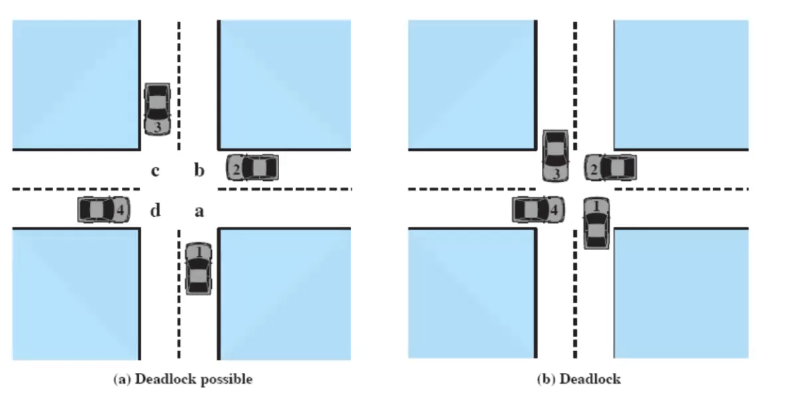
\includegraphics[width=0.5\textwidth]{immagini/DeadlockVItaComune}
    \caption{Deadlock}
    \label{fig:Deadlock}
\end{figure}
\begin{figure}[H]
    \centering
    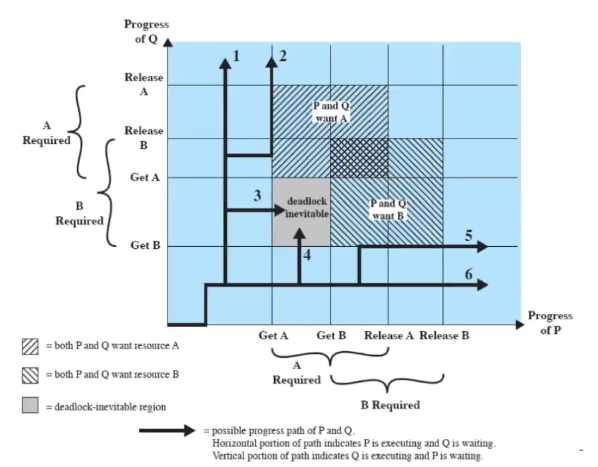
\includegraphics[width=0.5\textwidth]{immagini/JointProcessDiagram}
    \caption{Deadlock}
\end{figure}
Le situazioni di deadlock tra pochi processi possono essere analizzate con il joiont process diagram, che mostra
come due processi distinti sviluppano il loro procedimento in maniera congiunta, in questo grafico c'é una timeline
per un processo P e una per un processo Q, succede ad un certo punto che P dovra chiedere A e B, e lo stesso fara Q, da
notare che timeline di P e Q sono invertite, si vede che una risorsa viene rilasciata solo dopo che l'altra é stata richiesta,
grazie a questo diagramma possiamo quindi identificare i casi in cui il deadlock é possibile oppure certo, si vede che
si ha il deadlock quando un processo richiede accesso ad una risorsa ma l'altro processo le detiene entrambe, possiamo notare come
il deadlock possa essere casuale a seconda di come il dispatcher decide di eseguire i processi.
\begin{figure}[H]
    \centering
    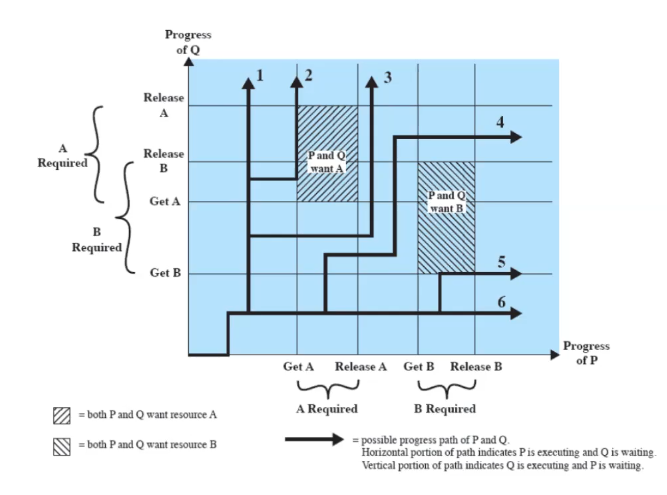
\includegraphics[width=0.5\textwidth]{immagini/JointProcessDiagramNoDeadlock}
    \caption{Deadlock}
\end{figure}
In questo caso non é possibile il deadlock, perché non c'é il caso in cui un processo detiene una risorsa e ne richiede
un'altra, contemporaneamente.
\subsection{Risorse Riusabili}
Per dare una caratterizzazione piú matematica dobbiamo prima fare una classificazione delle risorse, possiamo classificarle come:
\begin{itemize}
    \item \textbf{Risorse Riusabili}
    \item \textbf{Risorse Consumabili}
\end{itemize}
Le risorse riusabili sono risorse che possono essere usate da un solo processo alla volta, il fatto di essere usate non le consuma, ovvero
tutto ció che a che fare con la CPU,I/O channels, memoria primaria \dots ecc. una volta che un processo ottiene una risorse riusablie
prima o poi la rilascia, lo stallo avviene se un processo ha una risorsa e ne richiede un'altra prima di rilasciare la precedente.
\begin{figure}[H]
    \centering
    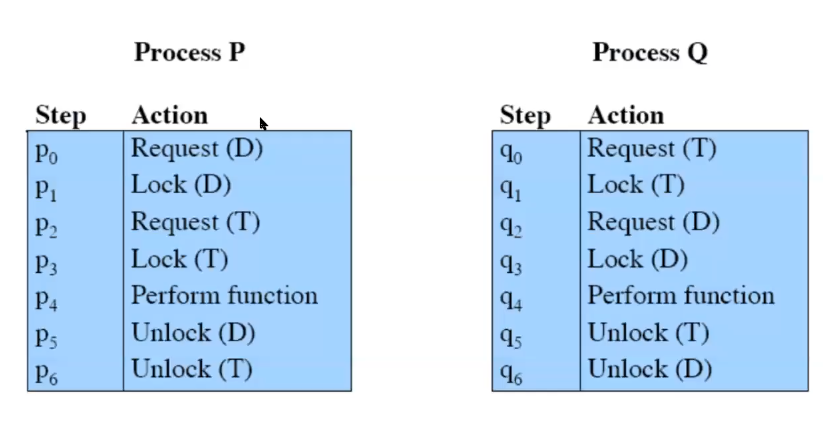
\includegraphics[width=0.5\textwidth]{immagini/EsempiRisorseRiusabili}
    \caption{Deadlock}
\end{figure}
\subsection{Risorse Consumabili}
Le risorse consumabili vengono create da un processo e distrutte da un altro, alcuni esempi sono interruzzioni,segnali,messaggi,informazioni nei
buffer, in questo caso si parla di deadlock perché un processo fa una richiesta su una risorsa ma quella risorsa non é ancora
stata creata.
\subsection{Allocazione delle Risorse}
Usando il grafo dell'allocazione delle risorse possiamo rappresentare i processi come cerche e le risorse come quadrati, il
grafo é un tipo di grafo diretto, i cui nodi sono divisi in due insiemi, uno per i processi e uno per le risorse, le risorse consumabili non mai
l'Held; invece i pallini compaiono e scompaiono, in generale il grafo funziona bene con le risorse riusabili.
\begin{figure}[H]
    \centering
    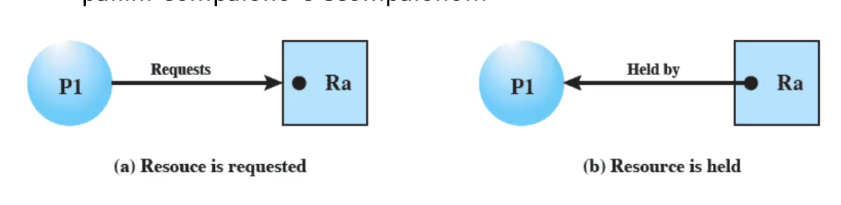
\includegraphics[width=0.5\textwidth]{immagini/GrafoAllocazioneDelleRisorse}
    \caption{Deadlock}
\end{figure}

\subsection{Condizioni di Deadlock per le risorse riusabili}
\begin{itemize}
    \item \textbf{Mutua Esclusione}: almeno una risorsa é non condivisibile, ovvero solo un processo alla volta puó usarla.
    \item \textbf{Hold and Wait}: un processo detiene una risorsa e ne richiede un'altra.
    \item \textbf{No Preemption}: le risorse non possono essere tolte ai processi, solo il processo che detiene la risorsa puó rilasciarla.
    \item \textbf{Circular Wait}: esiste un insieme di processi P1,P2,\dots,Pn tali che P1 detiene una risorsa che P2 richiede, P2 detiene una risorsa che P3 richiede e cosí via fino a Pn che richiede una risorsa che P1 detiene.
\end{itemize}
\subsection{Condizioni di Deadlock per le risorse consumabili}
\begin{itemize}
    \item \textbf{Mutua Esclusione}: la risorsa va a chi ne fa richiesta per primo poi viene distrutta.
    \item \textbf{Hold and Wait}: si puó richiedere una risorsa quando ancora non é stata creata.
    \item \textbf{No Preemption}: non appena una viene concessa un risorsa viene distrutta.
    \item \textbf{Circular Wait}: esiste un insieme di processi P1,P2,\dots,Pn tali che ciascun processo dovrebbe creare una risorsa (invano) dal processo che lo segue.
\end{itemize}
\begin{figure}[H]
    \centering
    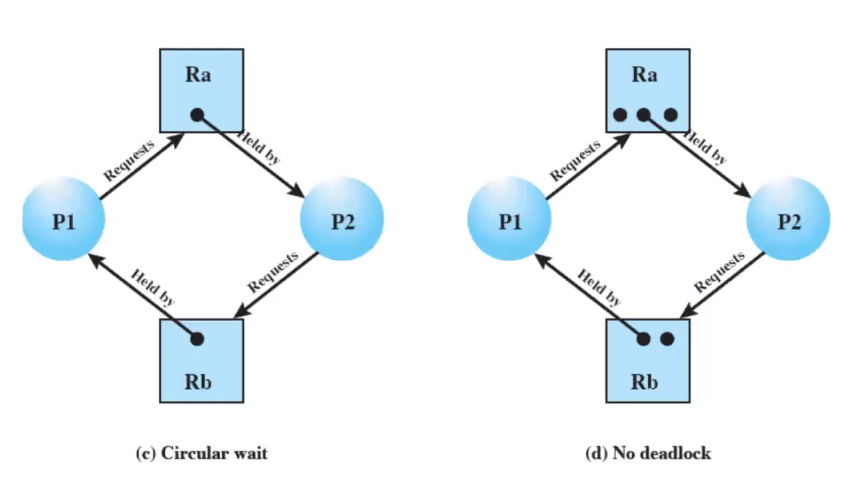
\includegraphics[width=0.5\textwidth]{immagini/GrafoAllocazioneDelleRisorseEsempio}
    \caption{Deadlock}
\end{figure}
\begin{figure}[H]
    \centering
    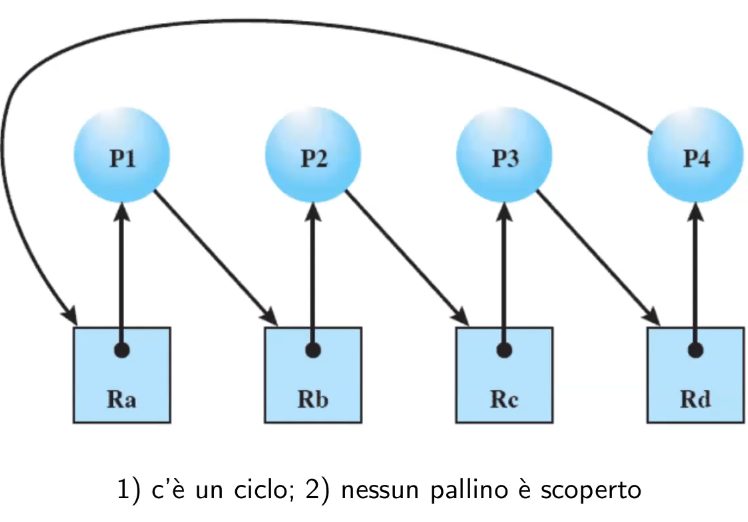
\includegraphics[width=0.5\textwidth]{immagini/GrafoAllocazioneDeiProcessiEsempioVitaComune}
    \caption{Traduzione in Grafo dell'esempio delle macchine}
\end{figure}
\subsection{Quando si verifica il Deadlock}
Abbiamo la possibilitá di avere un deadlock quando:
\begin{itemize}
    \item \textbf{Mutua Esclusione}: almeno una risorsa é non condivisibile, ovvero solo un processo alla volta puó usarla.
    \item \textbf{Hold and Wait}: un processo detiene una risorsa e ne richiede un'altra.
    \item \textbf{No Preemption}: le risorse non possono essere tolte ai processi, solo il processo che detiene la risorsa puó rilasciarla.
\end{itemize}
mentre si verifica il deadlock quando:
\begin{itemize}
    \item \textbf{Circular Wait}: esiste un insieme di processi P1,P2,\dots,Pn tali che P1 detiene una risorsa che P2 richiede, P2 detiene una risorsa che P3 richiede e cosí via fino a Pn che richiede una risorsa che P1 detiene.
\end{itemize}
Le prime tre condizioni non sono dovute all'esecuzione dei processi, ma a come é fatto in sistema
























